\documentclass{article}

\usepackage[final]{neurips}
\usepackage{listings}

\usepackage{multicol}
\usepackage{float}
\usepackage[center]{caption}

\usepackage[utf8]{inputenc} % allow utf-8 input
\usepackage[T1]{fontenc}    % use 8-bit T1 fonts
\usepackage{hyperref}       % hyperlinks
\usepackage{url}            % simple URL typesetting
\usepackage{booktabs}       % professional-quality tables
\usepackage{amsfonts}       % blackboard math symbols
\usepackage{nicefrac}       % compact symbols for 1/2, etc.
\usepackage{microtype}      % microtypography
\usepackage{graphicx}
\usepackage{amsmath}
\usepackage{xepersian}

\settextfont{XB Yas.ttf}

\title{
\lr{An Exploratory Assignment on Minimum Spanning Trees}\\
پروژه‌ی نهایی درس الگوریتم‌های تصادفی (شماره ۷)
}


\author{%
  امیرحسین مهدی‌نژاد\\
  شماره دانشجویی ۸۱۰۸۰۰۰۵۸\\
  \texttt{mahdinejad@ut.ac.ir} \\
   \And
  حسین پیرهادی\\
  شماره دانشجویی ۸۱۰۸۰۰۰۳۷\\
  \texttt{hossein.pirhadi@ut.ac.ir}
}

\begin{document}


\begin{minipage}{0.1\textwidth}% adapt widths of minipages to your needs

\includegraphics[width=1.1cm]{Photos/UT_logo.png}
\end{minipage}%
\hfill%
\begin{minipage}{0.9\textwidth}\raggedleft
دانشکده فنی، دانشگاه تهران\\
الگوریتم‌های تصادفی -  
تیر
ماه ۱۴۰۱\\
\end{minipage}
% \end{}

\makepertitle

% ---------- PROBLEM DESCRIPTION ----------
\section{شرح مسئله}
یک گراف کامل بدون جهت با
$\binom{n}{2}$
یال داریم.
هر یال وزنی حقیقی به صورت تصادفی با توزیع یکنواخت در بازه‌ی
$\left[0,1\right]$
دارد.

هدف ما بررسی نحوه‌ی رشد وزن مورد انتظار درخت کمینه‌ی پوشا و تخمین آن به شکل تابعی از
$n$
برای گراف است.
این کار مستلزم پیاده‌سازی یک الگوریتم یافتن درخت کمینه‌ی پوشا و روشی برای ساخت یک گراف تصادفی مناسب است.

بسته به الگوریتمی که استفاده می‌کنیم و نحوه‌ی پیاده‌سازی، ممکن است با زیاد شدن
$n$
به مشکل حافظه برخورد کنیم؛ به همین علت، از این روش پیروی می‌کنیم: نامحتمل است که درخت کمینه‌ی پوشا، یالی با وزن بیشتر از
$k(n)$
داشته باشد. می‌توانیم 
$k(n)$
را با تکرار اجرای الگوریتم برای مقادیر کوچک
$n$
بدست آوریم و سپس هر یال سنگین‌تر از
$k(n)$
را وقتی
$n$
بزرگ است دور بیاندازیم. البته دور انداختن چنین یال‌هایی ممکن است باعث شود درخت پوشایی که پیدا می‌شود کمینه نباشد.

به ازای مقادیر
$n=16, 32, 64, 128, 256, 512, 1024, 2048, 4096, 8192$
و اگر سرعت به اندازه‌ی کافی مناسب بود برای مقادیر بیشتر نیز اجرا می‌کنیم.
حداقل ۵ بار به ازای هر
$n$
الگوریتم را اجرا کرده و میانگین می‌گیریم؛ جدولی بر اساس میانگین وزن درخت برای مقادیر مختلف
$n$
که به ازای آن‌ها الگوریتم با موفقیت اجرا می‌شود، ارائه می‌کنیم.

% ---------- IMPLEMENTATION DETAILS ----------
\section{پیاده‌سازی}
این پروژه شامل کدهای الگوریتم اصلی به زبان
\lr{c++}
و همچنین بررسی نتایج و رسم نمودارها به زبان
\lr{python}
است.
% --------------------------------------------------------
\subsection{متد مونت کارلو}
روش مونت کارلو به طور کل مبتنی بر شبیه‌سازی است؛ وقتی برای مسائل سخت راه‌حل معمولی پیدا نمی‌کنیم، می‌توانیم با استفاده از این روش تا حد خوبی به جواب نزدیک شویم. این روش ساده و معمولا (نه همیشه) سریع است اما قابلیت تعمیم ندارد، یعنی اگر به ازای پارامترهایی به نتیجه رسیده، نمی‌توانیم به طور قطع در مورد مسئله با پارامترهای متفاوت نظر بدهیم.

در مسئله‌ای که با آن مواجهیم، در هر مرحله گراف کاملی را بر اساس توضیحات بخش قبل، ساخته و آن را به الگوریتم یافتن درخت کمینه‌ی پوشا می‌دهیم.
با توجه به تعداد زیاد یال‌های موجود در گراف کامل، ایده‌ی اصلی این مسئله در واقع پیدا کردن حدی برای دور ریختن یال‌های اضافی و در نتیجه بالاتر بردن سرعت پیدا کردن درخت کمینه‌ی پوشاست. کافیست با شبیه‌سازی الگوریتم برای تعدادی نمونه، تابع مورد نظر را بیابیم و برای تعداد راس‌های بیشتر از آن استفاده کنیم.
% --------------------------------------------------------
\subsection{شبیه‌سازی الگوریتم اصلی}
توضیحات این بخش مربوط به فایل
\lr{mst\_kruskal.cpp}
است.
% --------------------------------------------------------
\subsubsection{اجرای تست‌ها}
در بدنه‌ی اصلی برنامه، به ازای هرکدام از مقادیر مختلف
\lr{test\_size}
تابع
\lr{make\_test}
را ۲۰ بار فراخوانی می‌کنیم که در آن تابع، وکتوری به سایز مد نظر، از
\lr{Edge}
ها ساخته می‌شود؛
\lr{Edge}
در واقع یک
\lr{struct}
برای نشان دادن یال بی‌جهت بین دو برچسب
\lr{u, v}
با وزن
\lr{weight}
است.

به صورت زیر یال‌های گراف کامل ما با استفاده از دو حلقه‌ی تو در تو، و با توزیع وزن‌های یکنواخت بین ۰ و ۱ ساخته می‌شود. بعد از تعیین یک تابع
$k(n)$
مناسب، این بخش از کد دستخوش تغییر خواهد شد:

\begin{latin} 
\begin{verbatim}
    vector<Edge> graph;

    for(int i=0; i<test_size; i++){
        for(int j=i+1; j<test_size; j++){
            double rnd = distribution(generator);
            graph.push_back((Edge){i, j, rnd});
        }
    }
\end{verbatim}
\end{latin}

محاسبه‌ی زمان صرف شده برای اجرای الگوریتم یافتن درخت کمینه‌ی پوشا روی گراف مد نظر، از تفاضل زمان پایان و زمان آغاز، به ترتیب بعد و قبل از فراخوانی تابع مذکور به این شکل انجام می‌شود:

\begin{latin} 
\begin{verbatim}
    clock_t start = clock();
    auto result = mst_kruskal(graph, test_size);
    clock_t end = clock();
\end{verbatim}
\end{latin}

در آخر، خروجی این تست به عنوان یک سطر در فایل
\lr{csv}
افزوده شده و مقادیر تعداد رئوس گراف، مجموع وزن درخت کمینه‌ی پوشا، ماکزیمم یال موجود در درخت کمینه‌ی پوشا و زمان صرف شده برای محاسبه‌ی درخت کمینه‌ی پوشا به ترتیب نوشته می‌شوند:

\begin{latin}
\begin{verbatim}
    output << test_size << ',' <<
                get<0>(result) << ',' <<
                get<1>(result) << ',' <<
                static_cast<double>((end-start))/CLOCKS_PER_SEC << '\n';
\end{verbatim}
\end{latin}
% --------------------------------------------------------
\subsubsection{تابع کروسکال}
خروجی تابع
\lr{mst\_kruskal}
یک تاپل سه‌تایی
\lr{tuple<double, double, vector<Edge> >}
به ترتیب شامل مجموع وزن درخت کمینه‌ی پوشا، ماکزیمم یال موجود در درخت کمینه‌ی پوشا و در نهایت وکتوری شامل یال‌های درخت است. ورودی‌های این تابع
\lr{vector<Edge> edges}
وکتوری شامل یال‌های گراف و
\lr{int n\_vertices}
تعداد رئوس هستند.

الگوریتم کروسکال در هر مرحله، کمینه‌ی یال‌هایی که تا کنون ندیده است را به نحوی که تشکیل دور ندهد، به گراف خروجی اضافه می‌کند. پس در هر مرحله یک جنگل پوشا داریم که در آغاز هریک از رئوس به تنهایی در درختی مستقل از این جنگل قرار گرفته و کم‌کم به یک درخت واحد خواهیم رسید. پس برچسب‌گذاری در ابتدا به این شکل انجام می‌پذیرد:

\begin{latin}
\begin{verbatim}
    vector<int> forest_label(n_vertices);
    iota(forest_label.begin(), forest_label.end(), 0);
\end{verbatim}
\end{latin}

اپراتور مقایسه‌ای که در ساختار
\lr{Edge}
تعریف شده، حکم
\lr{comparator}
برای مرتب‌سازی موجود در
$STL$
را دارد. لذا با دستور
\lr{sort(edges.begin(), edges.end())}
یال‌های گراف ورودی را به ترتیب صعودی وزن‌هایشان مرتب می‌کنیم.

\begin{latin}
\begin{verbatim}
    bool operator<(const Edge& edge){
        return weight < edge.weight;
    }
\end{verbatim}
\end{latin}

با در نظر گرفتن مقادیر
\lr{total = 0}
به عنوان مجموع هزینه‌ی درخت کمینه‌ی پوشا،
\lr{max\_edge = -1}
به عنوان ماکزیمم یال موجود در درخت کمینه‌ی پوشا و همچنین یک وکتور از یال‌ها به اسم
\lr{mst}،
ادامه‌ی روند الگوریتم را بررسی کرده و در خلال توضیحات به آن می‌پردازیم.

به ازای هر یال از گراف، اگر برچسب سر و ته آن یال در درخت‌های متفاوتی از جنگل قرار بگیرد، این یال باید به
$mst$
و در نتیجه وزن آن به
\lr{total}
افزوده شود.

\begin{latin}
\begin{verbatim}
    for(auto edge: edges){
        if(forest_label[edge.u] != forest_label[edge.v]){
            total += edge.weight;
            mst.push_back(edge);
\end{verbatim}
\end{latin}

اگر وزن یال مذکور از ماکزیمم وزنی که درخت کمینه‌ی پوشا به خود دیده است بیشتر بود، ماکزیمم را بروزرسانی می‌کنیم.

\begin{latin}
\begin{verbatim}
            if(edge.weight > max_edge)
                max_edge = edge.weight;
\end{verbatim}
\end{latin}

حال نوبت یکسان کردن برچسب دو سر تمامی یال‌های موجود در درخت کمینه‌ی پوشاست. طبیعتا به ازای هر راس، در صورتی که
\lr{old\_label}
را ببینیم بجای آن
\lr{new\_label}
خواهیم گذاشت.

\begin{latin}
\begin{verbatim}
            int old_label = forest_label[edge.u],
                new_label = forest_label[edge.v];
            for(int vertex=0; vertex<n_vertices; vertex++){
                if(forest_label[vertex] == old_label)
                    forest_label[vertex] = new_label;
            }
        }
    }
\end{verbatim}
\end{latin}

در نهایت خروجی را به شکل یک تاپل سه‌تایی
\lr{make\_tuple(total, max\_edge, mst)}
برمی‌گردانیم.
% --------------------------------------------------------
\subsection{بررسی نتایج و رسم نمودارها}
خروجی بدست آمده از بخش قبل به ازای ۲۰ بار اجرای الگوریتم برای تعداد رئوس بین ۲ تا ۱۰۲۴ در قالب یک فایل
\lr{csv}
به کد
\lr{conclusion.ipynb}
داده شد. با رسم ستون سوم (ماکزیمم وزن موجود در درخت کمینه‌ی پوشا) بر حسب ستون اول (تعداد رئوس گراف) چنین نموداری حاصل شد:

\begin{figure}[H]
    \centering
    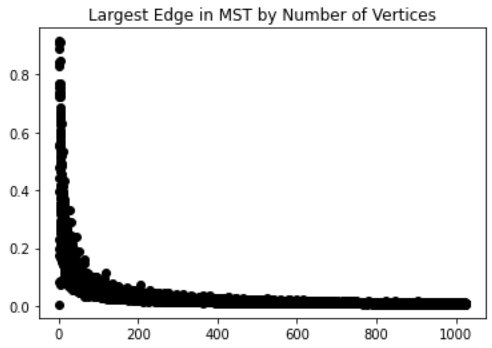
\includegraphics[width=0.6\linewidth]{Photos/Randomized mst/first_result.png}
    \caption{
    سنگین‌ترین یال موجود در درخت کمینه‌ی پوشا برحسب تعداد رئوس
    }
    \label{fig:my_label}
\end{figure}

با بررسی خروجی فایل اکسل، میانگین وزن درخت کمینه‌ی پوشا در حدود
$1.2$
بوده و بدین ترتیب می‌توان با حدس
$k(n)=\frac{1.2}{n}$
کار را آغاز کرد؛ اما خطای آن خیلی زیاد بوده و عملا برای تعداد رئوس زیاد کاربردی ندارد. زیرا به دنبال تابعی هستیم که تمامی نقاط این نمودار، پایین‌تر از آن قرار بگیرند تا بتوانیم وزن‌های بزرگ‌تر از آن مقدار را نادیده بگیریم.

طبیعتا هرچه فاصله‌ی تابع از نقاط ماکزیمم کمتر باشد، سرعت اجرای الگوریتم بالاتر رفته (تعداد یال‌های بیشتری کنار گذاشته می‌شوند) و از طرفی ریسک از دست دادن
\lr{mst}
واقعی بیشتر می‌شود. نحوه‌ی انتخاب
$k(n)$
در بخش آخر این گزارش توضیح داده شده است. حدس‌های زیادی با آزمون و خطاهای فراوان انجام شد که به دو مورد از آن‌ها با برچسب‌های
$k_1$
و
$k_2$
در اینجا اشاره خواهد شد.

$$k_1(n)=\frac{1.2\times(1-\epsilon)^{n-140}}{n^\delta\times\log(n)}, (\epsilon=0.001, \delta=0.1)$$

$$k_2(n)=0.04+\frac{(1-\epsilon)^n}{n^\delta\times\log_{\beta}(n)}, (\epsilon=0.008, \delta=0.05, \beta=4.5)$$

دوباره نمودار قبلی را این بار در کنار 
$k_1$
و
$k_2$
(به ترتیب خطوط آبی و قرمز رنگ) رسم می‌کنیم تا ضمن مقایسه‌ی این دو تابع، یکی را به عنوان حدس نهایی انتخاب کنیم.

\begin{figure}[H]
    \centering
    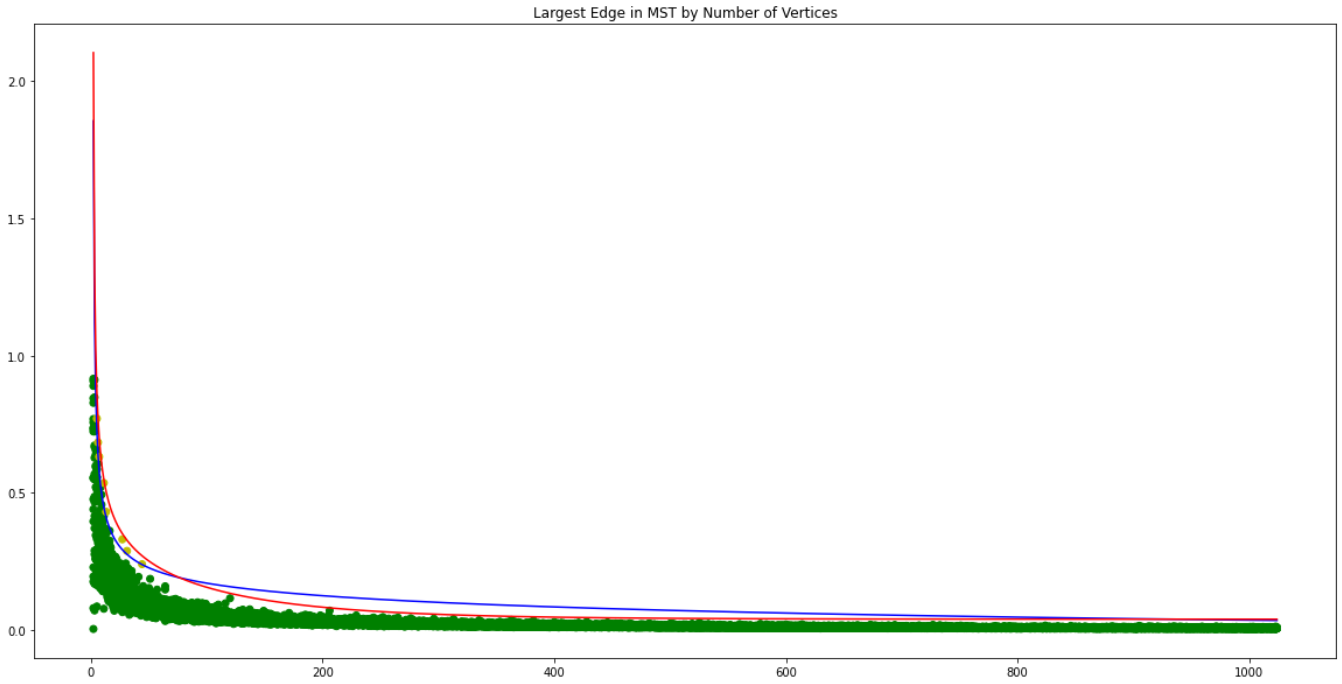
\includegraphics[width=0.999\linewidth]{Photos/Randomized mst/k_n_result.png}
    \caption{
    مقایسه‌ی
    $k_1$
    و
    $k_2$
    با روند تغییرات وزن سنگین‌ترین یال موجود در درخت کمینه‌ی پوشا برحسب تعداد رئوس
    }
    \label{fig:my_label}
\end{figure}

نقاط زرد رنگ نمودار فوق که تعداد آن‌ها در داده‌های مذکور ۸تا بوده، در واقع خطای تابع آبی‌رنگ هستند در صورتی که تابع قرمز رنگ روی این داده‌ها خطایی ندارد و حدس بهتری است؛ پس
$k_2$
را برای دور ریختن یال‌های اضافی استفاده خواهیم کرد.
% --------------------------------------------------------
\subsection{دور ریختن یال‌های سنگین‌تر}
با توجه به نتایج بدست آمده در بخش قبل، تابع مذکور را به صورت زیر پیاده‌سازی می‌کنیم:

\begin{latin}
\begin{verbatim}
double k(int n){
    return 0.04 + pow(0.992, n)/(pow(n, 0.05) * log(n)/log(4.5));
}
\end{verbatim}
\end{latin}

در مرحله‌ی ساخت گراف تصادفی، قبل از اینکه یالی را به وکتور یال‌ها اضافه کنیم بررسی می‌کنیم که وزن آن کمتر یا مساوی
$k(n)$
باشد.

\begin{latin}
\begin{verbatim}
            if(rnd <= k(test_size))
                graph.push_back((Edge){i, j, rnd});
\end{verbatim}
\end{latin}

تست به ازای توان‌های ۲ از عدد ۱۶ تا ۸۱۹۶ انجام شده، بقیه‌ی مراحل مثل قبل تکرار شده و در نهایت خروجی در فایل
\lr{result.csv}
نوشته خواهد شد.

میانگین زمان اجرا از
$0.214304$
ثانیه برای ۱۰۲۴ راس به
$0.007731$
ثانیه کاهش یافت که بسیار چشم‌گیر است؛ همچنین برای گراف ۸۱۹۲ راسی این مقدار در حدود
$0.653266$
ثانیه خواهد بود.

% ---------- CONCLUSION ----------
\section{نتیجه‌گیری}
\subsection{میانگین وزن درخت کمینه‌ی پوشا، با رشد 
$n$
چگونه تغییر می‌کند؟}
دامنه‌ی نوسانات هزینه‌ی درخت کمینه‌ی پوشا، مطابق با شکل زیر در حدود
$1.2$
قرار گرفته و با زیاد شدن تعداد رئوس نیز این روند ادامه پیدا می‌کند.

\begin{figure}[H]
    \centering
    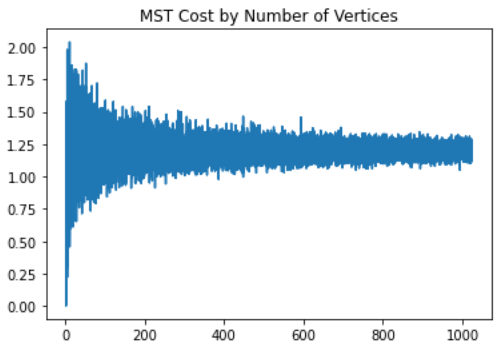
\includegraphics[width=0.6\linewidth]{Photos/Randomized mst/mst_cost.png}
    \caption{
    هزینه‌ی درخت کمینه‌ی پوشا بر حسب تعداد رئوس
    }
    \label{fig:my_label}
\end{figure}

میانگین هزینه‌ی درخت کمینه‌ی پوشا در ۲۰ بار اجرا، برحسب تعداد یال‌ها به صورت زیر بدست آمده است:

\begin{latin}
\begin{verbatim}
final_result.groupby(by='n_vertices').mean()['mst_cost']

16      1.212090
32      1.209557
64      1.185509
128     1.211534
256     1.186387
512     1.200954
1024    1.194176
2048    1.203449
4096    1.200361
8192    1.205207
\end{verbatim}
\end{latin}
% --------------------------------------------------------
\subsection{از کدام الگوریتم درخت کمینه‌ی پوشا استفاده کردیم و چرا؟}
الگوریتم کروسکال در موقعیت‌های معمولی یعنی برای گراف‌های
\lr{sparse}
عملکرد بهتری از خود نشان می‌دهد و همچنین از داده‌ساختار ساده‌تری استفاده می‌کند. از آنجا که بخش اعظمی از یال‌های گراف کامل را کنار گذاشته‌ایم و تراکم یال‌ها پایین است، کروسکال را انتخاب می‌کنیم.
% --------------------------------------------------------
\subsection{زمان اجرای الگوریتم چقدر است؟}
در اینجا طبق توضیحات بخش‌های قبلی گزارش، ساده‌ترین پیاده‌سازی کروسکال مورد استفاده قرار گرفته که پیچیدگی آن از مرتبه‌ی
$O(E\log(E)+V^2)$
است که در آن
$E\log(E)$
برای مرتب‌سازی یال‌ها بوده و
$V-1$
بار عملیات اجتماع گرفتن بین درخت‌های مختلف از جنگل، هر کدام با مرتبه‌ی
$V$
انجام می‌شود.

\begin{latin}
\begin{verbatim}
final_result.groupby(by='n_vertices').mean()['time_spent']

16      0.000030
32      0.000089
64      0.000161
128     0.000223
256     0.000617
512     0.001912
1024    0.007731
2048    0.033999
4096    0.151774
8192    0.653266
\end{verbatim}
\end{latin}


میانگین زمان صرف شده برای یافت درخت کمینه‌ی پوشا، به ازای
$V$
های مختلف، به شکل فوق به‌دست آمده است.

% --------------------------------------------------------
\subsection{اگر بنا بر دور ریختن یال‌ها باشد، چگونه به نحوی تاثیرگذار
$k(n)$
را تعیین کنیم؟}
می‌توان از مدل‌های مختلف یادگیری ماشین یا روش‌های یافتن پوش سیگنال استفاده کرد. در اینجا ما صرفا با آزمون و خطا، ضرایب مختلف را امتحان کرده و به نتیجه رسیدیم.

ابتدا با حدس
$\frac{1.2}{\log{n}}$
شروع کردیم و با مشاهده‌ی اینکه نقاط دیتاست از این تابع فاصله دارند، یک
$n^\delta$
در مخرج ضرب کرده و با بالا و پایین کردن مقدار دلتا، مقدار مناسب آن را پیدا می‌کنیم. از آنجا که می‌خواهیم ابتدای نمودار کمی بالاتر و هرچقدر
$n$
زیاد می‌شود نمودار پایین‌تر بیاید،
$(1-\epsilon)^{n-140}$
را در صورت ضرب می‌کنیم و به
$k_1$
می‌رسیم.

پایه‌ی لگاریتم مخرج روی دوری یا نزدیکی کنج نمودار به داده‌ها، و توان
$n$
روی چولگی نمودار تاثیرگذارند. تفاوت عمده‌ی
$k_2$
با
$k_1$
در واقع اضافه کردن مقدار
$0.04$
است که حد این عبارت برای
$n$
های بزرگ را تعیین می‌کند.
% --------------------------------------------------------
\subsection{بدون اثبات دقیق، چه توضیحی برای نتایج بدست آمده ارائه می‌کنید؟}
از آنجا که هزینه‌ی درخت کمینه‌ی پوشا همیشه در حدود
$1.2$
است، هرچقدر تعداد رئوس بیشتر می‌شود باید وزن یال‌های موجود در این درخت کمتر شده باشد چون حدودا همان مقدار را این بار بین یال‌های بیشتری تقسیم می‌کنیم.

توزیع وزن‌ها به صورت یکنواخت انجام شده است، با تعیین یک حد مناسب می‌توان اکثریت یال‌ها
[
که اتفاقا کمترین نقش را در درخت کمینه‌ی پوشا دارند
]
را از محاسبات کنار گذاشت. در واقع همین یکنواخت بودن توزیع به ما امکان استفاده از متد مونت کارلو را می‌دهد.

با توجه به توضیحات بخش قبل، راه‌حل ارائه شده یک راه‌حل کاربردی در دنیای واقعیست و گرچه ممکن است همیشه درخت کمینه را برنگرداند ولی با توجه به سرعت بسیار بیشتر و فضای ذخیره سازی بسیار کمتر، در عمل کاربردی است.

\begin{table}[htb]

    \centering % instead of \begin{center}
    \caption{مقایسه‌ی وزن مورد انتظار درخت کمینه‌ی پوشا بین الگوریتم ما و الگوریتم معمولی}
    \vspace{2mm} % Adjust the height of the space between caption and tabular

    \begin{tabular}{ | l | l | l | l | l | l | l |}
        \hline
        \lr{n\_vertices}  & $256$ & $512$ & $1024$ & $2048$ & $4096$ & $8192$ \\ \hline
        \lr{naive algorithm} & $1.1873$ & $1.1859$ & $1.2121$ & $1.1985$ & $1.2052$ & $1.2033$ \\ \hline
        \lr{this assignment} & $1.1863$ & $1.2009$ & $1.1941$ & $1.2034$ & $1.2003$ & $1.2052$ \\ \hline
    \end{tabular}

\end{table}
% --------------------------------------------------------
\subsection{چه تجربه‌ای از کار با مولد اعداد تصادفی دارید و آیا قابل اطمینان است؟}
به طور خاص در مورد زبان
\lr{c++}
که در این پروژه مورد استفاده قرار گرفته،
\lr{rand}
را یک
\lr{pseudorandom number generator}
می‌نامند که به
\lr{seed}
وابسته بوده و این برای کاربردهایی که در آن‌ها امنیت مهم است، چیز بدیست.

از طرفی وقتی رندومی بین صفر تا
\lr{RAND\_MAX}
دلخواهی تولید می‌شود و آن‌را به
$x$
باقی‌مانده می‌گیریم، مگر در صورتی که
\lr{RAND\_MAX}
مضربی از
$x$
باشد، یکنواخت نیست.

\begin{latin}
\begin{verbatim}
    random_device randomDevice;
    default_random_engine generator(randomDevice());
    uniform_real_distribution<double> distribution(0.0, 1.0);
\end{verbatim}
\end{latin}

اما در ورژن‌های ۱۱ به بعد
\lr{c++}
برای تولید رندوم یکنواخت بین ۰ تا ۱، با توجه به قطعه کد فوق، به شکل
\lr{rnd = distribution(generator)}
عمل می‌کنیم.
% --------------------------------------------------------

\end{document}